\documentclass[12pt]{article}
\usepackage{geometry}
\usepackage{graphicx} % 插图
\usepackage{float} % 插图位置固定
\usepackage{amsmath} % 文字加粗
\usepackage[UTF8]{ctex} %中文宏包
\setCJKmainfont{SimSun}
\usepackage{fontspec} %引入字体设置宏包
\setmainfont{Times New Roman}
\usepackage{indentfirst} %首行缩进
\usepackage{listings} %代码
\usepackage{color} %字体颜色
\usepackage{subfigure}  %插入多图时用子图显示的宏包

\usepackage{minted} %代码
\usemintedstyle{vs}


%\usepackage{fancyhdr} %页眉页脚
%\pagestyle{fancy} 
%\fancyhf{}
%\lhead{数字图像处理}
%\chead{Noise Reduction Using a Median Filter}
%\rhead{张青铭 \quad 3200105426}
%\renewcommand{\headrulewidth}{0pt}
%图片路径
\graphicspath{ {figures/} }

%页面格式
\geometry{a4paper,
left=20mm,
right=20mm,
top=20mm,
bottom=20mm }

\title{{\Huge{\textbf{数字图像处理}}}\\Pro9-1\quad  Morphological and Other Set Operations}
\author{信息与电子工程学院\quad 信息工程 \quad 3200105426\\张青铭}
\date{\today}

\begin{document}
\maketitle
\section{实验任务}
(1)编写程序,可以指定大小为3*3的任意结构元素进行二值膨胀和侵蚀;

(2)编写一个用于执行集合交集、差分和互补的程序;
\section{算法设计}
1.腐蚀与膨胀:

因为题目要求结构元大小为3*3,所以需要先对图像外围增加一圈0,再对图像元素进行遍历。腐蚀计算公式$ A \oplus B=\{z|(\hat B)_z \cap A \neq\emptyset \} $和膨胀计算公式为$ A \ominus B=\{ z|(B)_z \subseteq A\} $,程序中利用结构元与对应像素值的并获得每一点的值。
\\

2.交集、差分和互补;

使用矩阵的为逻辑运算即可得到。
\section{代码实现}
\begin{minted}[frame=lines,tabsize=4,python3,baselinestretch=0.85]{matlab}
%%腐蚀与膨胀
function [imd,ime]= Erode_Dilation(ima,A)
	%ima为输入图像,A为输入的3*3结构元
	%imd为输出的膨胀图,ime为输出的腐蚀图
	[m,n]=size(ima);
	imd=ones(m,n);
	ime=zeros(m,n);
	p=zeros(3,3);
	q=zeros(3,3);
	%将输入图像四周添加一圈0元素
	imb=zeros(m+2,n+2);
	for i=2:m+1
		for j=2:n+1
			imb(i,j)=ima(i-1,j-1);
		end
	end
	for i=2:m+1
		for j=2:n+1
			%膨胀计算
			p=A&[imb(i-1,j-1),imb(i-1,j),imb(i-1,j+1);
				 imb(i,j-1),imb(i,j),imb(i,j+1);
				 imb(i+1,j-1),imb(i+1,j),imb(i+1,j+1)];
				if (p==zeros(3,3))
					imd(i-1,j-1)=0;
				end
			%腐蚀计算
			q=A&[imb(i+1,j+1),imb(i+1,j),imb(i+1,j-1);
				 imb(i,j+1),imb(i,j),imb(i,j-1);
				 imb(i-1,j+1),imb(i-1,j),imb(i-1,j-1)];
			if (q==A)
				ime(i-1,j-1)=1;
			end
		end
	end
end
%%交集、差分和互补
img\_inter=img1&img2;
img\_differ=img1&(~img2);
img\_complete=~img1;
%%主程序
clear;close all;clc;
SE=ones(3,3);%结构元
img1_ones=255*ones(339,338);%全1图
img2_zeros=zeros(1294,1247);%全0图
img1=imread('fig1.tif');
img2=imread('fig2.tif');
%腐蚀与膨胀
[imd1,ime1]=Erode_Dilation(img1,SE);
[imd2,ime2]=Erode_Dilation(img2,SE);
%交集、差分和互补
img1_inter=img1_ones&img1;
img1_differ=img1_ones&(~img1);
img1_complete=~img1;
img2_inter=img2_zeros&img2;
img2_differ=img2_zeros&(~img2);
img2_complete=~img2;
%作图
figure(1)
subplot(131);imshow(img1);title('original');
subplot(132);imshow(imd1);title('dilate');
subplot(133);imshow(ime1);title('erode');
figure(2)
subplot(131);imshow(img2);title('original');
subplot(132);imshow(imd2);title('dilate');
subplot(133);imshow(ime2);title('erode');
figure(3)
subplot(131);imshow(img1_inter);title('inter')
subplot(132);imshow(img1_differ);title('differencing')
subplot(133);imshow(img1_complete);title('completment')
figure(4)
subplot(131);imshow(img2_inter);title('inter')
subplot(132);imshow(img2_differ);title('differencing')
subplot(133);imshow(img2_complete);title('completment')
\end{minted}

\section{实验结果}
1.腐蚀与膨胀

分别取两张图做腐蚀与膨胀结果如下:
\begin{figure}[H]
	\centering
	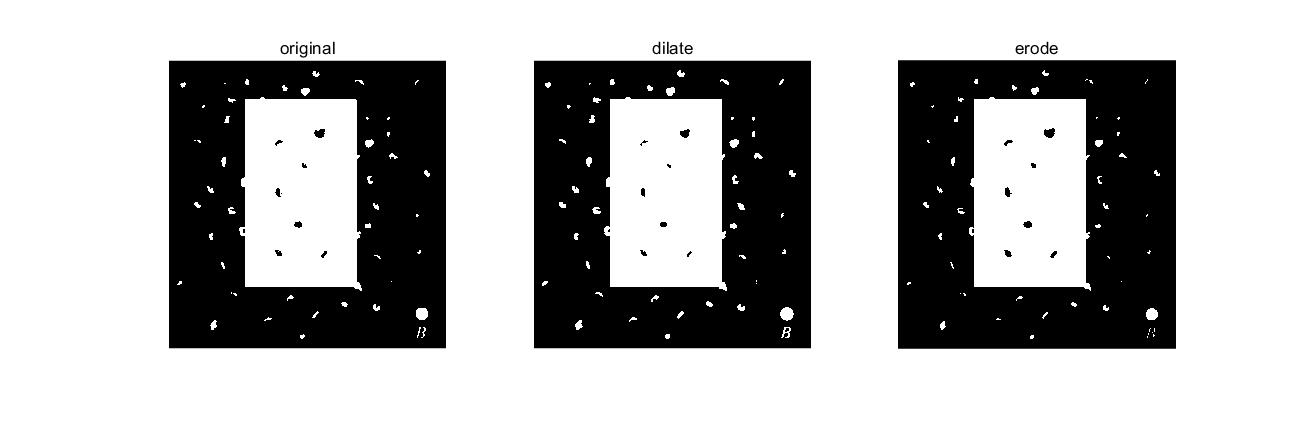
\includegraphics[width=1\linewidth]{figures/ed1}
	\caption{第一组}
\end{figure}
\begin{figure}[H]
	\centering
	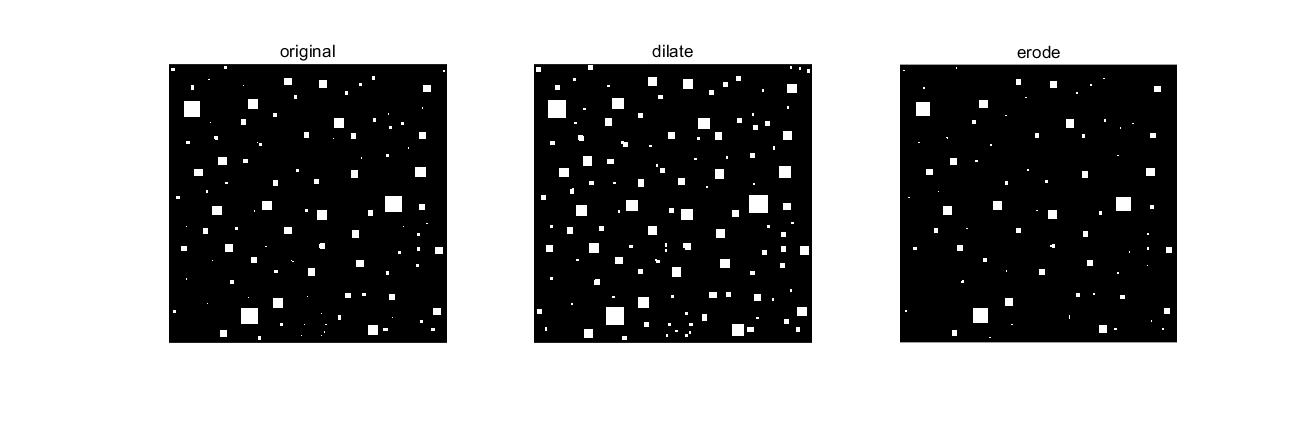
\includegraphics[width=1\linewidth]{figures/ed2}
	\caption{第二组}
\end{figure}

由于原图像较大,3*3的结构元处理效果并不明显,但仍能观察到腐蚀与膨胀处理后相较于原图的差异。膨胀后图像前景被放大,腐蚀后前景缩小并且一些部分更加“割裂”。
\\

2.交集、差分和互补

将图1与全1的图进行交集、差分和互补的结果如下:
\begin{figure}[H]
	\centering
	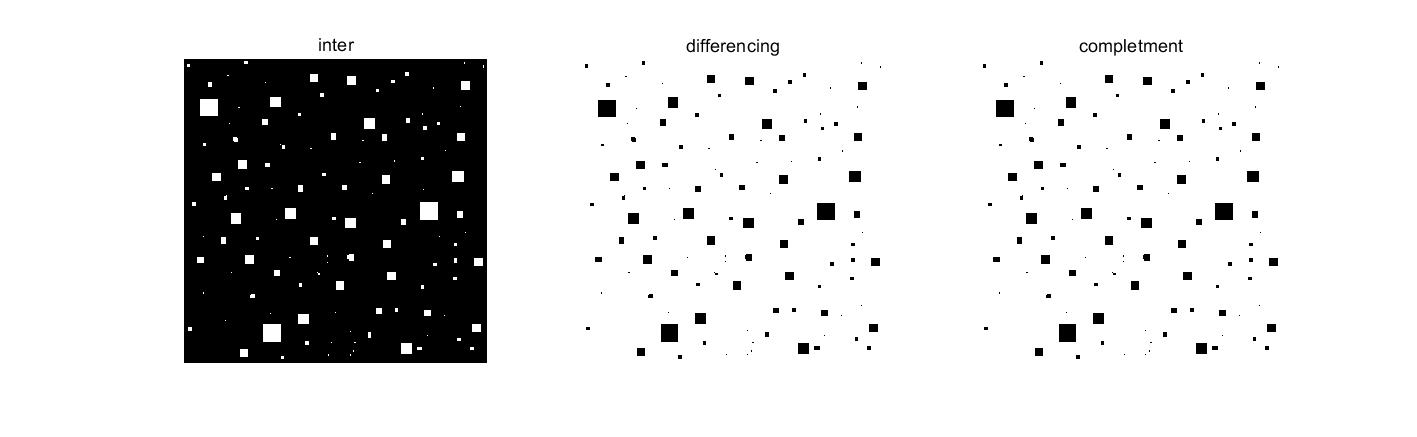
\includegraphics[width=0.8\linewidth]{figures/2}
	\caption{与全1图像交差补}
\end{figure}

可以发现交集为原图像没有改变,差分为白色和黑色翻转,互补也为白色和黑色翻转,均符合理论预期。

将图2与全0的图进行交集、差分和互补的结果如下:
\begin{figure}[H]
	\centering
	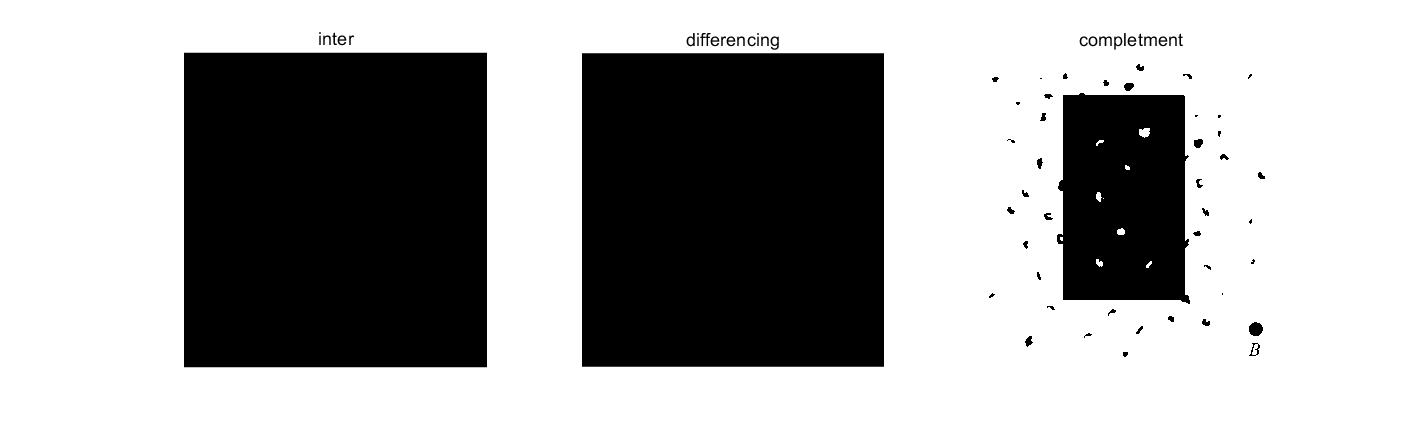
\includegraphics[width=0.8\linewidth]{figures/1}
	\caption{与全0图像交差补}
\end{figure}

可以发现交集为全黑图像,差分也为全黑图像,互补也为白色和黑色翻转,也均符合理论预期。
\section{总结}
本次实验对形态学的基本操作腐蚀和膨胀进行了实现,实现方法用了最简单的遍历法,比较简单。但如果将结构元取大,仍用该方法会导致在计算部分比较繁琐,对于图像局部像素的取出会比较麻烦。但总体上思想比较简单。同时也对二值图像的集合运算进行了实现。因为没有很好的相适应的两张图像,所以只与全1图和全0图进行了操作,最后结果也符合预期。总的来说这次实验比较简单,并且内容结果很直观。
\end{document}
